%!TEX root=paper.tex
\section{Evaluation}

The goal of our evaluation is to explore (1) whether, by varying $\lambda$,
\shrink can efficiently explore (in terms of number of training runs)  the
spectrum of high-accuracy models from small to large, on both CNNs and fully
connected networks.  Our results show that, for each network size, we obtain
models that perform as well or better than \textit{Static Networks}, trained via
traditional hyperparameter optimization;  (2) whether, because these  smaller
networks are dense, they result in improved inference times on both CPUs and
GPUs; and (3) whether the \shrink approach results in network architectures that
are substantially different than the best network architectures (in terms of
relative number of neurons per layer) identified in the literature.

\noindent\textbf{Implementation: }We implemented \swls and
the associated training procedure as a library in
pytorch~\cite{paszke2017automatic}. The layer can be freely mixed with other
popular layers such as convolutional layers, batchnorm layers, fully connected
layers, and used with all the traditional optimizers. We use our implementation
to evaluate \shrink throughout the evaluation section.

\subsection{Can \shrink achieve good accuracy?}
%\subsection{Performance vs. Traditional Methods}

To answer this question we compare \shrink with a traditional network. In both
cases, we need to perform hyperparameter optimization to explore different
network architectures. We perform random search, which is an effective technique
for this purpose \cite{BergstraJAMESBERGSTRA2012}. We evaluate \shrink on two
well-known datasets. One for which it is not possible to explore the entire
space of network architectures (\texttt{CIFAR10}) and one for which it is
possible to do so (\texttt{COVERTYPE}).

\noindent\textbf{Setup: } We assume no prior knowledge on the optimal batch
size, learning rate, $\lambda$ or weight decay ($\lambda_2$). Instead, we
trained a number of models, randomly and independently selecting the values of
these parameters from a range of reasonable values. Training is done using
gradient descent and the \textit{Adam} optimizer
\cite{DBLP:journals/corr/KingmaB14}. Specifically, we start with randomly
sampled learning
rate; for every $5$ epochs of non-improvement in validation
accuracy we divide the learning rate by $10$. We stop training after $400$
epochs or when the learning rate is under $10^{-7}$, whichever comes first. For
each of the models we trained, we pick the epoch with the best validation
accuracy and report the corresponding testing accuracy. Because of the nature of
our method, it can happen that for networks that are aggressively compressed,
the best validation accuracy is obtained early in training, before the size has
converged. To be sure that accuracy measured corresponds to the final shape and
not the starting shape, we only consider the second half of the training when
picking the best epoch. For each model, we also measure the total size, in terms
of number of floating point parameters, excluding the \swls because as described
in \cref{neuron_killing}, these are eliminated after training.


\subsubsection{Large Network Setting: \texttt{CIFAR10}}


\texttt{CIFAR10} is an image classification dataset containing $60000$ color
images $(3 \times 32 \times 32)$, belonging to $10$ different classes. We use it
with the \texttt{VGG16} network \cite{Srivastava2014}, which consists of
alternating convolutional layers and \textit{MaxPool} layers interleaved by
\textit{BatchNorm} \cite{DBLP:journals/corr/IoffeS15} and \textit{ReLU}
\cite{Nair2010} layers. The two last layers are fully connected layers
separated by a \textit{ReLU} activation function.

We applied \shrink to the VGG16 network by adding \swls
after each \textit{BatchNorm} layer and each fully connected layer (except the
last). Recall that \shrink assume that the starting size of the network is
an upper bound on the optimal size. Thus, we started with a
network with 2x the recommended size for each layer as an upper bound (this
is larger than what ImageNet uses). 

We compare against classical (\textit{Static}) networks. In such networks, the
number of parameters that control the size is large: 13 parameters for the
convolutional layers and $2$ for the fully connected layers. \shrink
effectively fuse all these parameters in a single $\lambda$, but in conventional
architectures where all of these parameters are free, it is infeasible to obtain
a reasonable sample of a search space of this size. For this reason, we rely on
the conventional heuristic that the original VGG architecture (and many CNNs)
use, where the number of channels is doubled every after \textit{MaxPool} laxer.
For \textit{Static Networks} we sample the size between $0.1$ and $2$ times the size
original one, optimized for ImageNet. We report the same numbers as we did for
\shrink and we compare the two distributions. 

The results are shown in the top figure of \cref{figure_CIFAR10}, with blue dots
indicating models produced by \shrink and orange dots indicating static networks. 
For each
model, we plot its accuracy and model size. The lines show the Pareto frontier
of models in each of the two optimization settings. \shrink explore the
trade-off between model size and accuracy more effectively. 

Note that the best performing \shrink model has $92.07\%$ accuracy which
is identical to the accuracy of the static network, while the \shrink model
is $2.22$ times smaller. In addition, if we give up just 1\% error, \shrink
find a model that is 35.5 times smaller than any static network that performs
as good or better.

\subsubsection{Small Network Setting: \texttt{COVERTYPE}}

The \texttt{COVERTYPE} \cite{Blackard:1998:CNN:928509} dataset contains $581012$
descriptions of geographical area (elevation, inclination, etc...) and the goal
is to predict the type of forest growing in each area. We picked this dataset
for two reasons. First it is simple, such that we can reach good accuracy with
only a few fully-connected layers. This is important because we want to show
that \shrink find sizes as good as \textit{Static Networks}, even if
we are sampling the entire space of possible network sizes. Second, Scardapane
et al~\cite{Scardapane2017} perform their evaluation on this dataset, which
allows us to compare the results obtained by our method with the method in
~\cite{Scardapane2017}.

%The experimental setup on this dataset is similar to {\tt CIFAR10}. 
We compare \shrink against the same architecture
used in \cite{Scardapane2017}, i.e., a three fully-connected layers network with no
\textit{Dropout} \cite{Srivastava2014} and no \textit{BatchNorm}. 
%\gl{Should we say
%here that we don't expect Dropout to work here ? I could write an entire
%paragraph about it if needed}. 
In this case, for the \textit{Static Networks}, we independently sample the
sizes of the three different layers to explore all possible architectures.

The results are shown in the top figure of \cref{figure_COVER}, with the two
optimization methods plotted as before. Here, {\it Static} method finds models
that perform well at a variety of sizes, because it is able to explore the
entire parameter space.  This is as expected;  the fact that \shrink perform
as well as Static indicates that \shrink are doing an effective job of
exploring the parameter space using just the single $\lambda$ parameter.

Note that the best performing \shrink models have $96.91\%$ accuracy while the
best static model is only $96.66\%$ accurate, while the \shrink model is $2.51$
times smaller. In addition, if we give up just 0.5\% error, \shrink find a
model that is 38.6 times smaller than any static network with equivalent accuracy.


\subsubsection{Summary}

We  demonstrated that it is possible to achieve networks with good accuracy
when using \shrink both when the network space cannot be explored entirely
(\texttt{CIFAR10}) and when it can, e.g., \texttt{COVERTYPE}. The most important
result is not that \shrink find networks of good accuracy, but that those
networks are much smaller than those found by a static method. The impact of the
network size on inference time is the subject of our next evaluation goal.


\subsection{Can ShrinkNets speed up inference?}

The previous experiment showed that \shrink find networks of similar or better accuracy
than static networks that are much smaller. We now explore if the reduction in size
translates into an improvement of the inference time.

As noted in the introduction, for some applications, compact models that offer
fast inference times are as important as absolute accuracy. 

%This observation motivates our 
% the experiment approach described in the previous section 
% and shown in the top of Figure~\ref{figure_CIFAR10} 
% and~\ref{figure_COVER}:
% for a  desired target accuracy, the Pareto optimal line shows the smallest
% network
% that satisfies achieves a given accuracy. 

In this section, we study the relationship between accuracy, network size and
inference time.  To do this, we select the smallest model that achieves a given
accuracy for the both \shrink and Static approach.  For each model, we measure
the time to run inference with the model.  We then compute the ratio of the
network size and inference time between \shrink and Static at each accuracy
level, and plot them on the bottom of Figure~\ref{figure_CIFAR10}
and~\ref{figure_COVER}.  We limit our plots to the models with $80-100\%$
accuracy range because those are the ones that we consider to be practically
useful.

The middle plot in each figure shows the ratio of model size between \shrink
and Static (values $>$1 mean \shrink are smaller) at different accuracy levels.
These figures show that is that size improvements are are particularly
significant for  \texttt{CIFAR10}. In the range of accuracies we are interested
in, improvements in size go from 4x to 40x. On the \texttt{COVERTYPE} dataset,
the compression ratio is always above 1 but it rarely exceeds 3x, except for
very high accuracies where \shrink find excellent, small solutions.  The fact
that the  \texttt{COVERTYPE} networks are not dramatically smaller is expected:
as the distribution at the top of Figure~\ref{figure_COVER} shows, the static
method is able to explore most of the parameter search space, so finds a range
of models that perform well at different sizes.

For speedup, we experimented with both CPUs and GPUs, and with different batch
sizes, where batch size indicates the number of inputs simultaneously fed to the
model for inference.  For each data set/GPU/CPU combination, we show results
with batch size 1, as well as with a batch size large enough to fully utilize
the hardware on each dataset and hardware configuration.  For example, for {\tt
CIFAR10} on CPU, a batch size of 64 fully utilizes the CPU, whereas a GPU can
execute many more models in parallel, so we use a larger batch size of 1024.
For {\tt COVERTYPE}, because the model is so much smaller, larger batches are
needed to fully utilize the hardware.  Note that when using a batch size of $1$
on GPU, we do not expect to (and do not) observe any improvement because
inference times are very small (typically about 10 $\mu s$), such that setup
time dominates overall runtime.  

The bottom four graphs in each figure show the results.  Again, the {\tt
CIFAR10} results show the benefit of the \shrink approach most dramatically.  On
CPU, speedups range up to 6x depending on the batch size, with many models
exceeding 3x speedup. In general, speedups are less than compression ratios, due
to overheads in problem setup, invocation, and result generation  in
Python/PyTorch.  On GPU, the speedups are less substantial because the CUDA
benchmarking utility that we use for evaluation can choose better algorithms for
larger matrices which masks some of our benefit, although they are still often
1.5x--2x faster for large batch sizes.  The speedup results on {\tt COVERTYPE}
are similar to those for network size:  because the networks are not much
smaller, they are not much faster either.

A key takeaway of these speedup results is that, unlike local sparsity
compression methods, our methods' improvement on size translates directly to
higher throughput at inference time~\cite{Han2015}.


\begin{figure*}[tb]\centering
\begin{minipage}{2.7in}
\centering
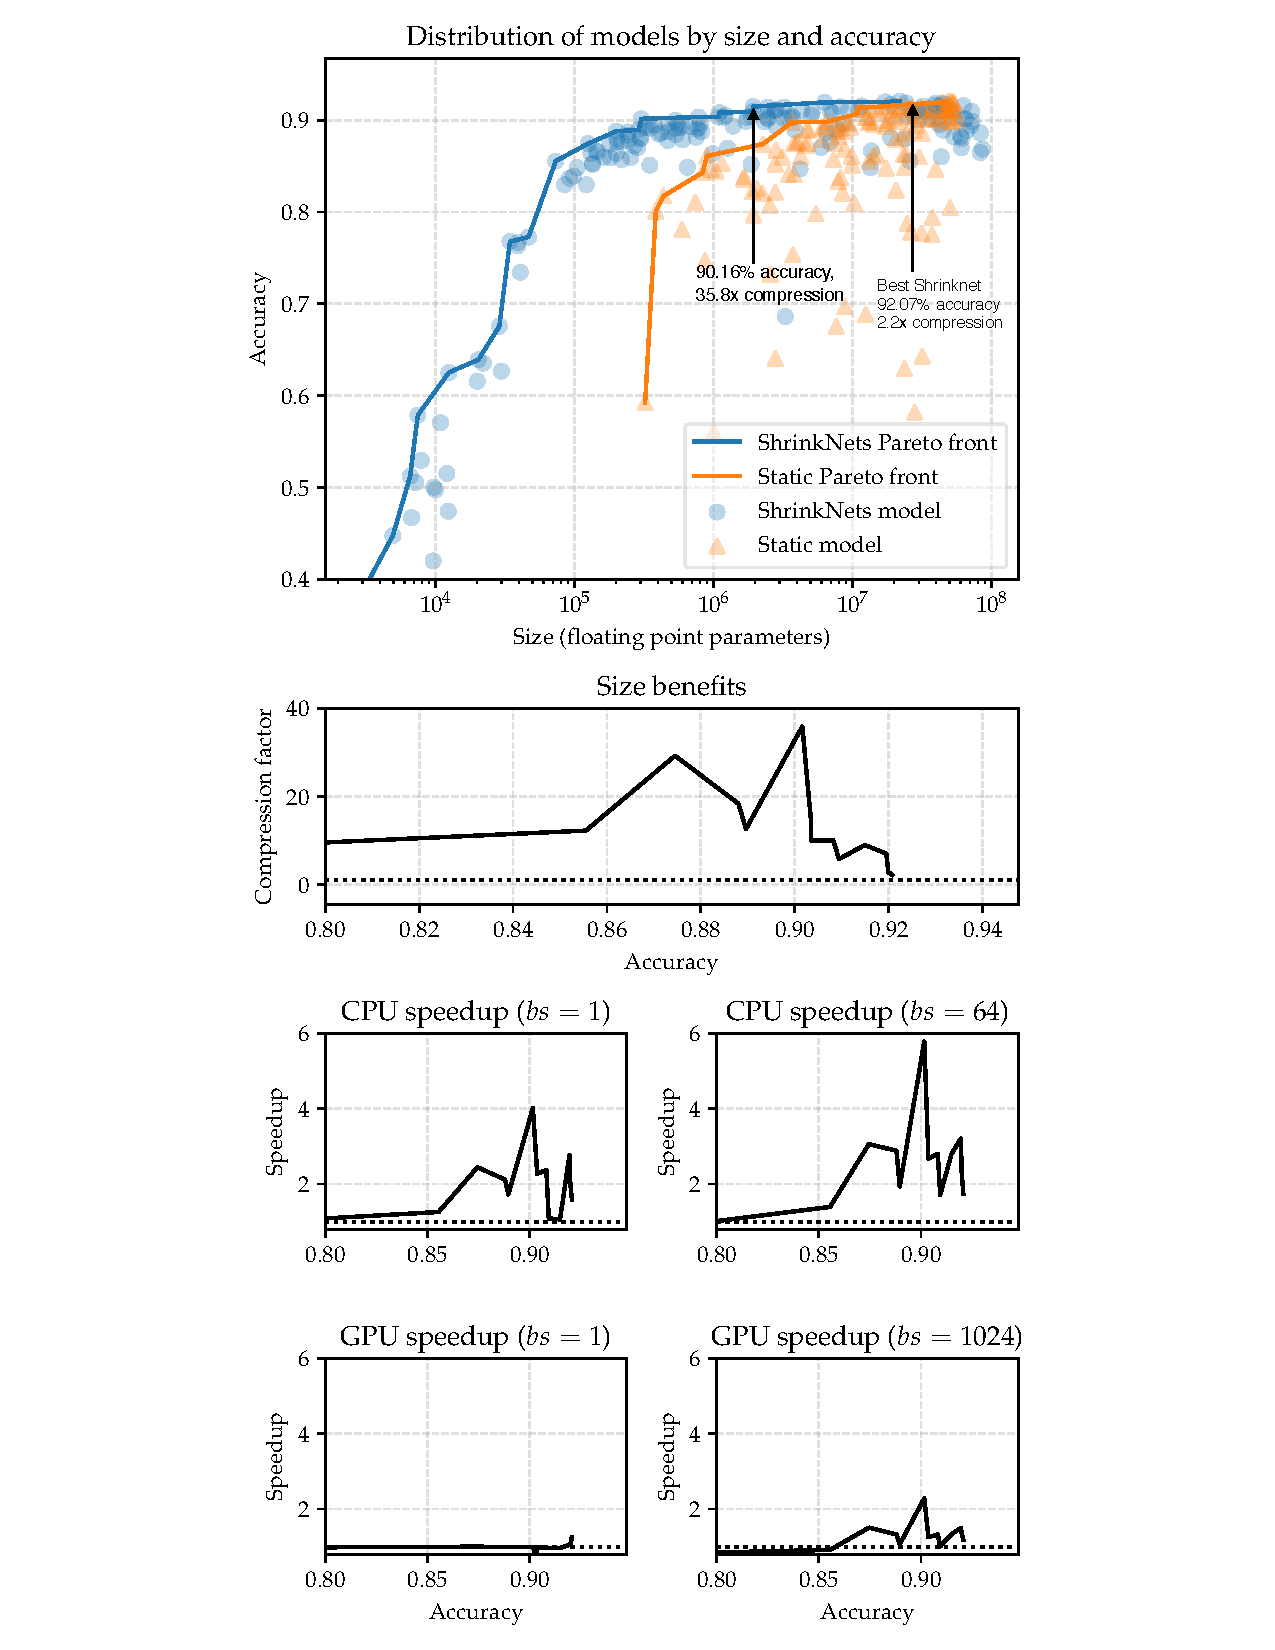
\includegraphics[width=\columnwidth]{CIFAR10_VGG_summary-arrows}
\vspace*{-10mm}
\caption{\label{figure_CIFAR10} Summary of the result of random
search over the hyper-parameters the \texttt{CIFAR10} dataset}
\vspace*{-5mm}
\end{minipage}
\begin{minipage}{.3in}
~~
\end{minipage}
\begin{minipage}{2.7in}
\centering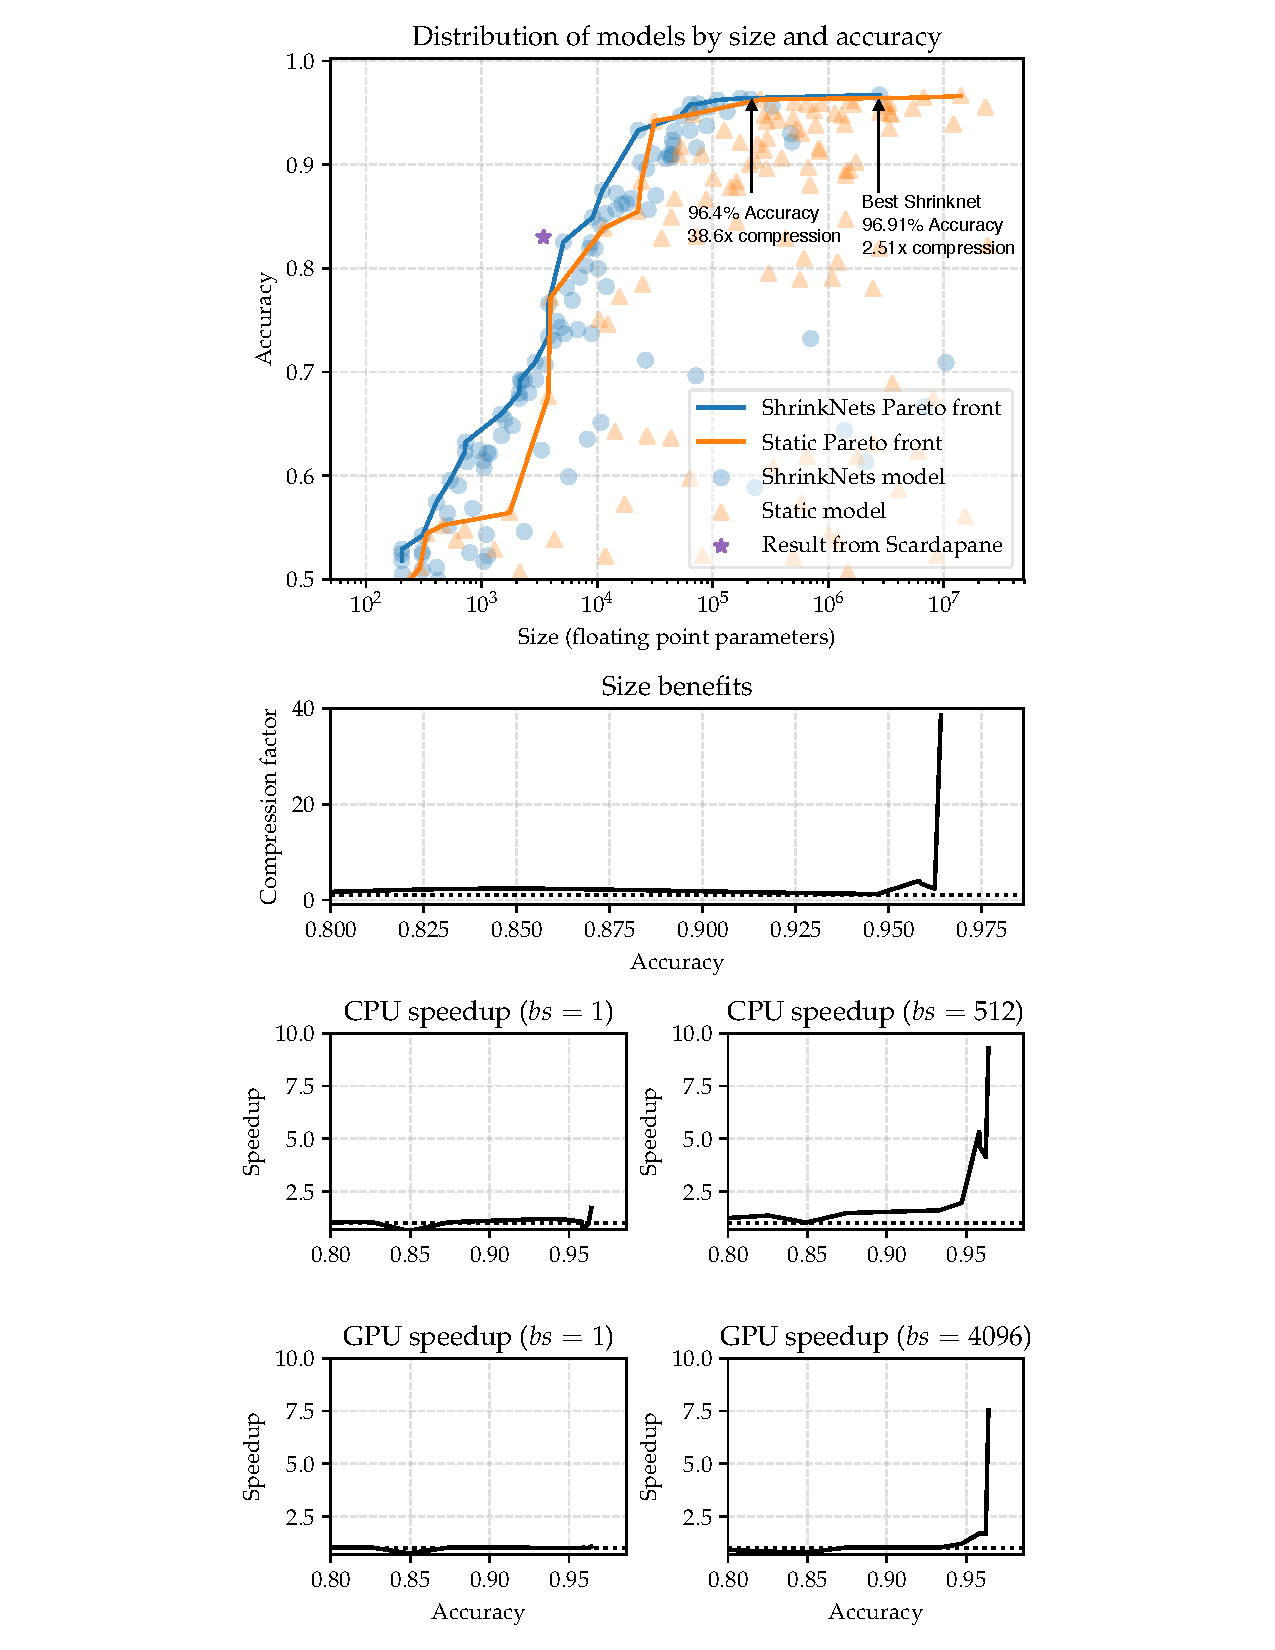
\includegraphics[width=\columnwidth]{COVER_FC_summary-arrows}
\vspace*{-10mm}
\caption{\label{figure_COVER} Summary of the result of random
search over the hyper-parameters the \texttt{COVERTYPE} dataset
}
\vspace*{-5mm}
\end{minipage}
\end{figure*}


\subsection{Architectures obtained after convergence}
\shrink effectively explore the frontier of model size and accuracy. For a
given target accuracy, the size needed is significantly smaller than when we use the
"channel doubling" heuristic commonly used to size convolutional neural networks.
This suggests that this conventional heuristic may not in fact be optimal,
especially when looking for smaller models.  Empirically we observed this to
often be the case.  For example, during our experimentations on the
\texttt{MNIST} \cite{Lecun1998} and \texttt{FashionMNIST} \cite{Xiao2017}
datasets (not reported here due to space constraints), we observed that even
though these datasets have the same number of classes, input features, and
output distributions, for a fixed $\lambda$ \shrink converged to
considerably bigger networks in the case of \texttt{FashionMNIST}. This evidence
shows that optimal architecture not only depends on the output distribution or
shape of the data but actually reflects the dataset.  This makes sense, as
\texttt{MNIST} is a much easier problem than \texttt{FashionMNIST}.

To illustrate this point on a larger dataset, we show two examples of
architectures learned by \shrink in
Figure~\ref{fig:network_size_evolution}.  The right arrow shows the model with the
best test accuracy, with identical performance to the best static
network; the left arrow shows a network that slightly under-performs the best in
terms of accuracy but is significantly smaller that the best equivalent
\textit{Static Network}.  In the plot, the dashed line
shows the number of neurons in each layer of the original VGG net, and the
shaded regions show the size of the \shrink as it converges (with the darkest
region representing the fully converged network).  Observe that the final
network that is trained looks quite different in the two cases, with the optimal
performing network appearing similar to the original VGG net, whereas the
shrunken network allocates many fewer neurons to the middle layers, and then
additional neurons to the final fewer layers.


\begin{figure}[h]
\begin{center}
\vspace{-.1in}
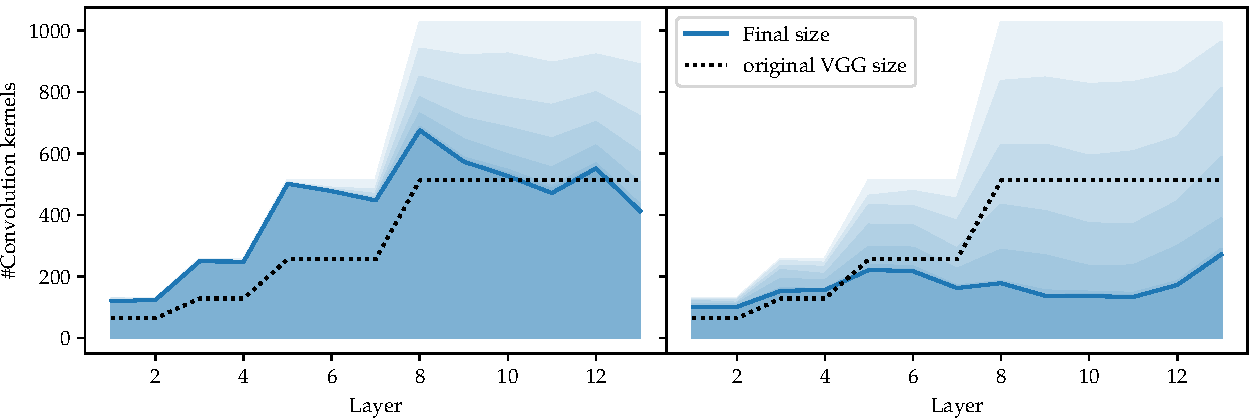
\includegraphics[width=.6\columnwidth]{size_evolution}
\vspace*{-5mm} 
\caption{ Evolution of the size of
  each layer over time (lighter: beginning, darker: end). On top a very large
  network performing $92.07\%$, at the bottom a simpler model with $90.5\%$
  accuracy. 
} 
\label{fig:network_size_evolution}
\end{center}
\vspace*{-4mm}
\end{figure}


